% ============================================================
% Filtros Pasa-altas (High-Pass)
% ============================================================
\section{Filtros Pasa-altas (High-Pass)}

\subsection{Butterworth}

\begin{figure}[H]
	\centering
	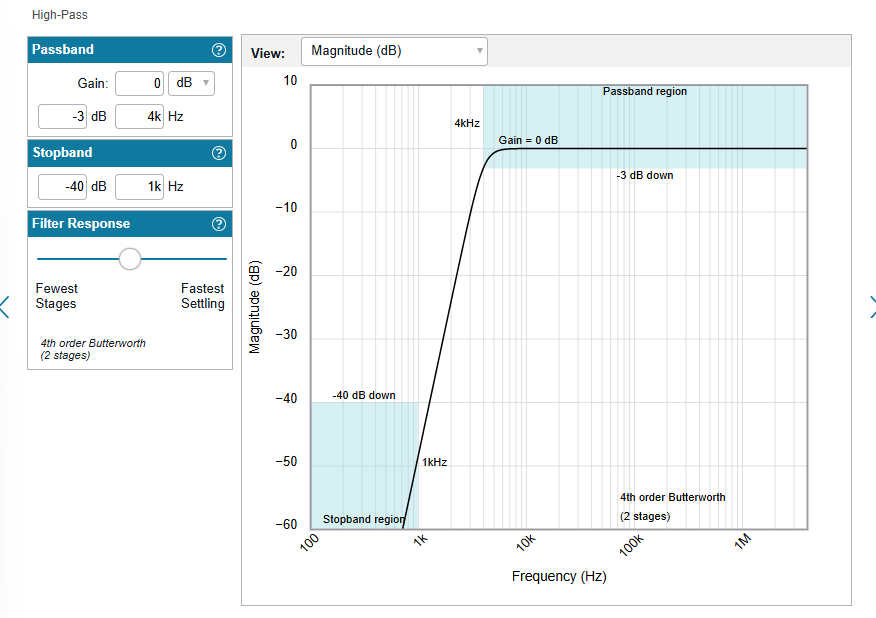
\includegraphics[width=0.9\textwidth]{img/hp_butterworth_respuesta.png}
	\caption{Respuesta en magnitud del filtro pasa-altas Butterworth de 4.\textsuperscript{o} orden.}
	\label{fig:hp_butterworth_respuesta}
\end{figure}

\begin{figure}[H]
	\centering
	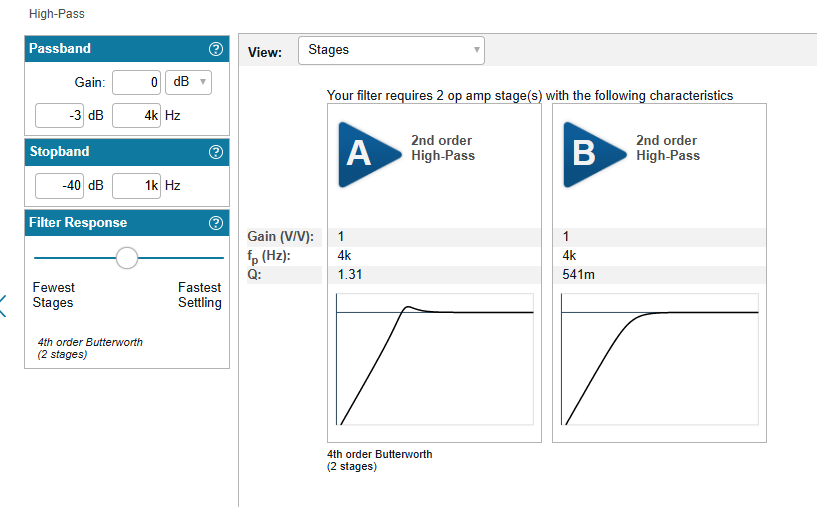
\includegraphics[width=0.9\textwidth]{img/hp_butterworth_etapas.png}
	\caption{Configuración de etapas (\textit{Stages}) del filtro pasa-altas Butterworth: dos etapas de segundo orden.}
	\label{fig:hp_butterworth_etapas}
\end{figure}

\begin{figure}[H]
	\centering
	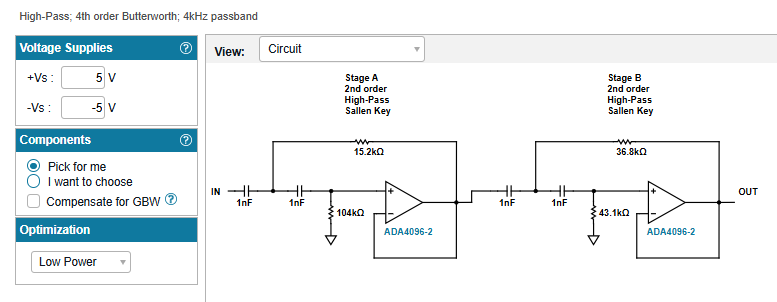
\includegraphics[width=\textwidth]{img/hp_butterworth_circuito.png}
	\caption{Circuito del filtro pasa-altas Butterworth.}
	\label{fig:hp_butterworth_circuito}
\end{figure}

% ------------------------------------------------------------
\subsection{Chebyshev}

\begin{figure}[H]
	\centering
	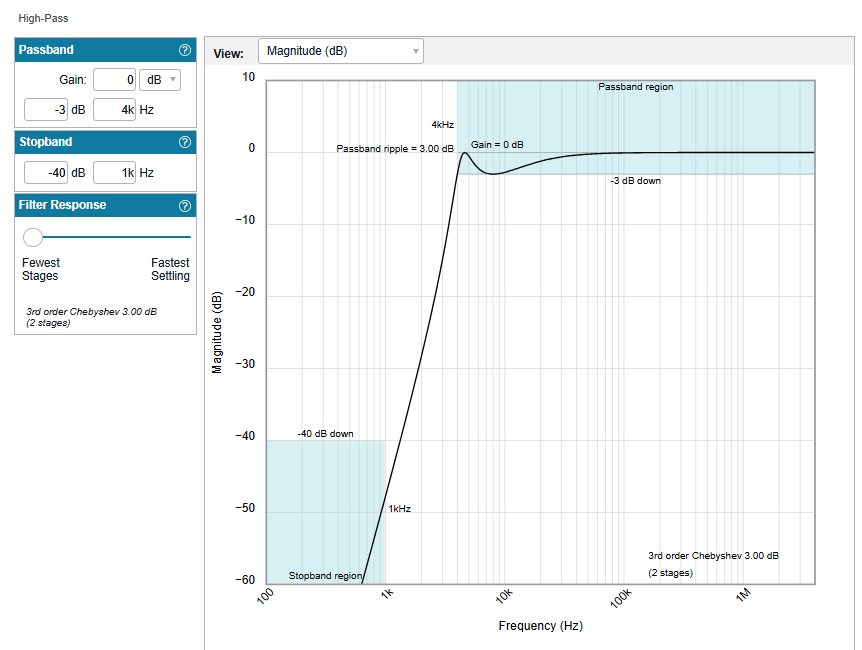
\includegraphics[width=0.9\textwidth]{img/hp_chebyshev_respuesta.png}
	\caption{Respuesta en magnitud del filtro pasa-altas Chebyshev de 3.\textsuperscript{er} orden (rizo de 3\,dB en la banda de paso).}
	\label{fig:hp_chebyshev_respuesta}
\end{figure}

\begin{figure}[H]
	\centering
	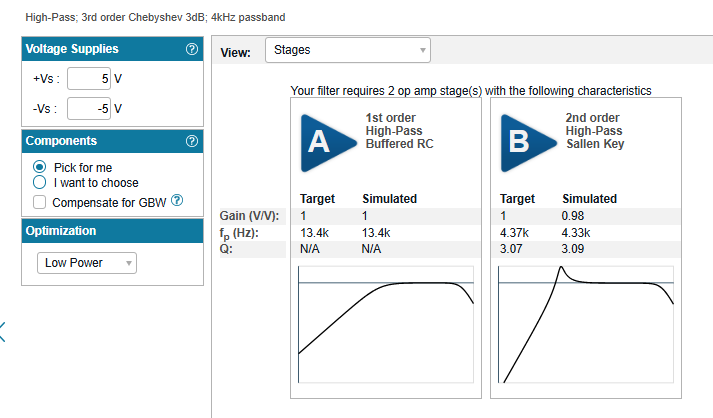
\includegraphics[width=0.9\textwidth]{img/hp_chebyshev_etapas.png}
	\caption{Configuración de etapas (\textit{Stages}) del filtro pasa-altas Chebyshev.}
	\label{fig:hp_chebyshev_etapas}
\end{figure}

\begin{figure}[H]
	\centering
	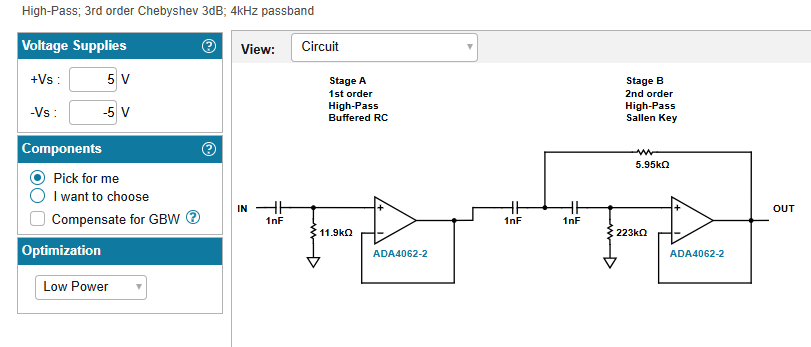
\includegraphics[width=\textwidth]{img/hp_chebyshev_circuito.png}
	\caption{Circuito del filtro pasa-altas Chebyshev.}
	\label{fig:hp_chebyshev_circuito}
\end{figure}

% ------------------------------------------------------------
\subsection{Bessel}

\begin{figure}[H]
	\centering
	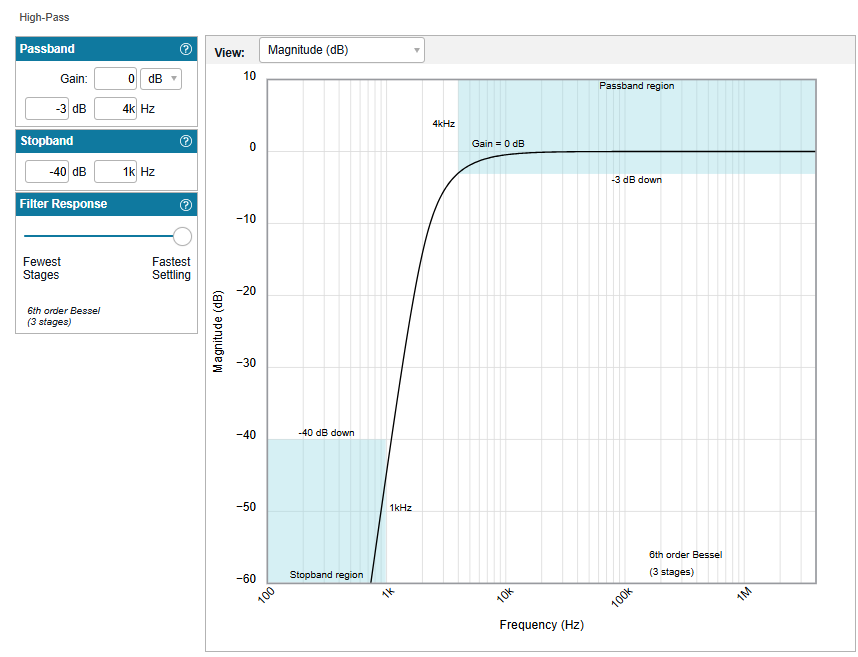
\includegraphics[width=0.9\textwidth]{img/hp_bessel_respuesta.png}
	\caption{Respuesta en magnitud del filtro pasa-altas Bessel de 6.\textsuperscript{o} orden.}
	\label{fig:hp_bessel_respuesta}
\end{figure}

\begin{figure}[H]
	\centering
	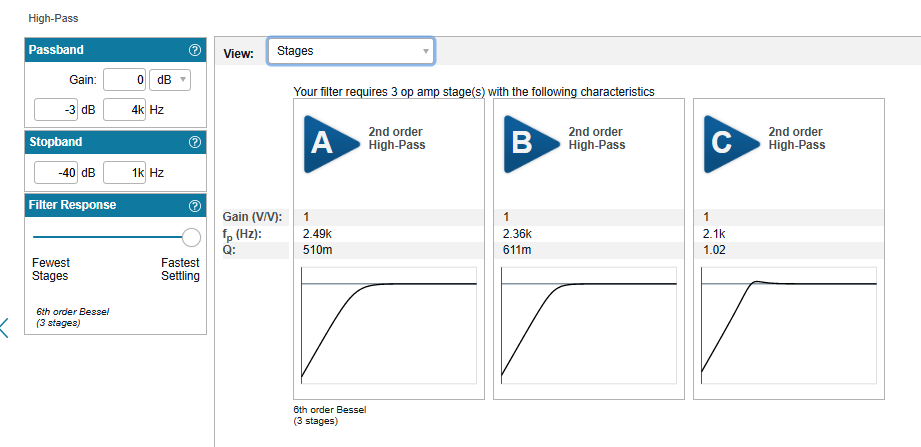
\includegraphics[width=0.9\textwidth]{img/hp_bessel_etapas.png}
	\caption{Configuración de etapas (\textit{Stages}) del filtro pasa-altas Bessel: tres etapas de segundo orden.}
	\label{fig:hp_bessel_etapas}
\end{figure}

\begin{figure}[H]
	\centering
	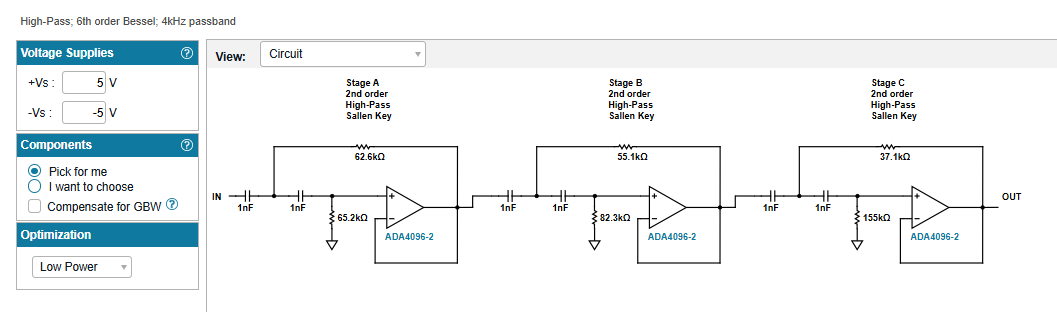
\includegraphics[width=\textwidth]{img/hp_bessel_circuito.png}
	\caption{Circuito del filtro pasa-altas Bessel.}
	\label{fig:hp_bessel_circuito}
\end{figure}
